\documentclass[
    amsfonts,
    amssymb,
    amsmath,
    preprint,
    floatfix,
    nofootinbib,
    aps,
    prl
]{revtex4-2}

\newcommand{\ManuscriptPdfTitle}{Supplemental Material for Amplitude-Robust Qubit Spectroscopy Using Echo-Root-Lorentzian Pulse Shapes}
% Encoding and language
\usepackage[T1]{fontenc}
\usepackage[utf8]{inputenc}
\usepackage[english]{babel}

% Mathematics
\usepackage{amsthm}
\usepackage{mathtools}
\usepackage{physics}

% Figures and layout
\usepackage{graphicx}
\usepackage{adjustbox}
\usepackage{placeins}
\usepackage{xcolor}

% Quotations
\usepackage{csquotes}

% Load hyperlinks last so package patches are applied consistently.
\providecommand{\ManuscriptPdfTitle}{Amplitude-Robust Qubit Spectroscopy Using Echo-Root-Lorentzian Pulse Shapes}
\usepackage[
    hidelinks,
    pdftitle={\ManuscriptPdfTitle},
    pdfauthor={Asaf A. Solonnikov and Nadav Katz}
]{hyperref}

\usepackage{float}

\begin{document}

\title{\texorpdfstring{Supplemental Material for\\
``Amplitude-Robust Qubit Spectroscopy Using Echo-Root-Lorentzian Pulse Shapes''}
{Supplemental Material for Amplitude-Robust Qubit Spectroscopy Using Echo-Root-Lorentzian Pulse Shapes}}

\author{Asaf A. Solonnikov and Nadav Katz}
\affiliation{The Racah Institute of Physics, The Hebrew University of Jerusalem, Israel}

\date{\today}
\maketitle

\setcounter{secnumdepth}{2}

This Supplemental Material provides the experimental setup, the Bloch-equation
coherence limit, pulse-cutoff and pulse-duration analyses, the adiabatic-basis
derivation, high-resolution and extended-amplitude scans, the numerical model,
a comparison of the root-Lorentzian and echo-root-Lorentzian protocols across
pulse parameters, and a comparison between simulation and experiment.

\renewcommand{\thesection}{S\arabic{section}}
\renewcommand{\thesubsection}{S\arabic{section}.\arabic{subsection}}
\renewcommand{\theequation}{S\arabic{equation}}
\renewcommand{\thefigure}{S\arabic{figure}}
\renewcommand{\thetable}{S\arabic{table}}

\section{Measurement Setup}
\label{sec:measurement-setup}

Experiments were performed on a QPU comprising 11 uncoupled superconducting
qubits hosted in a dilution refrigerator.  Control and readout were implemented
with a Quantum Machines OPX1000 equipped with a microwave front-end module
(MW-FEM), together with external cryogenic attenuators, filters, circulators,
and amplifiers.

A schematic of the setup is shown in Fig.~\ref{fig:diagram}.  The MW-FEM uses
direct digital synthesis and digital upconversion: a programmed complex pulse
envelope is translated to the configured microwave carrier and emitted directly
from an RF output, without an external analog local oscillator or IQ mixer
\cite{qm_opx1000_mwfem}.  For acquisition, the returned microwave signal is
digitally downconverted to a complex baseband stream.  QUA demodulation then
applies cosine and sine integration weights to the sampled signal and accumulates
the result to obtain the measured quadratures \cite{qm_opx_demodulation}.  Thus,
separate MW-FEM outputs provide the qubit-drive and resonator-readout tones,
while an MW-FEM input acquires the returning readout signal.  A dedicated DC
bias line was available but was not used in these measurements; consequently,
the qubits were not necessarily operated at their flux sweet spots.

The device was mounted at the mixing-chamber stage ($\sim$9 mK), with the drive
and readout lines attenuated across the refrigerator stages.  The returning
readout signal passed through circulators and a 4 K high-electron-mobility
transistor (HEMT) amplifier before entering the MW-FEM for digital
downconversion and demodulation.


\begin{figure}
    \centering
    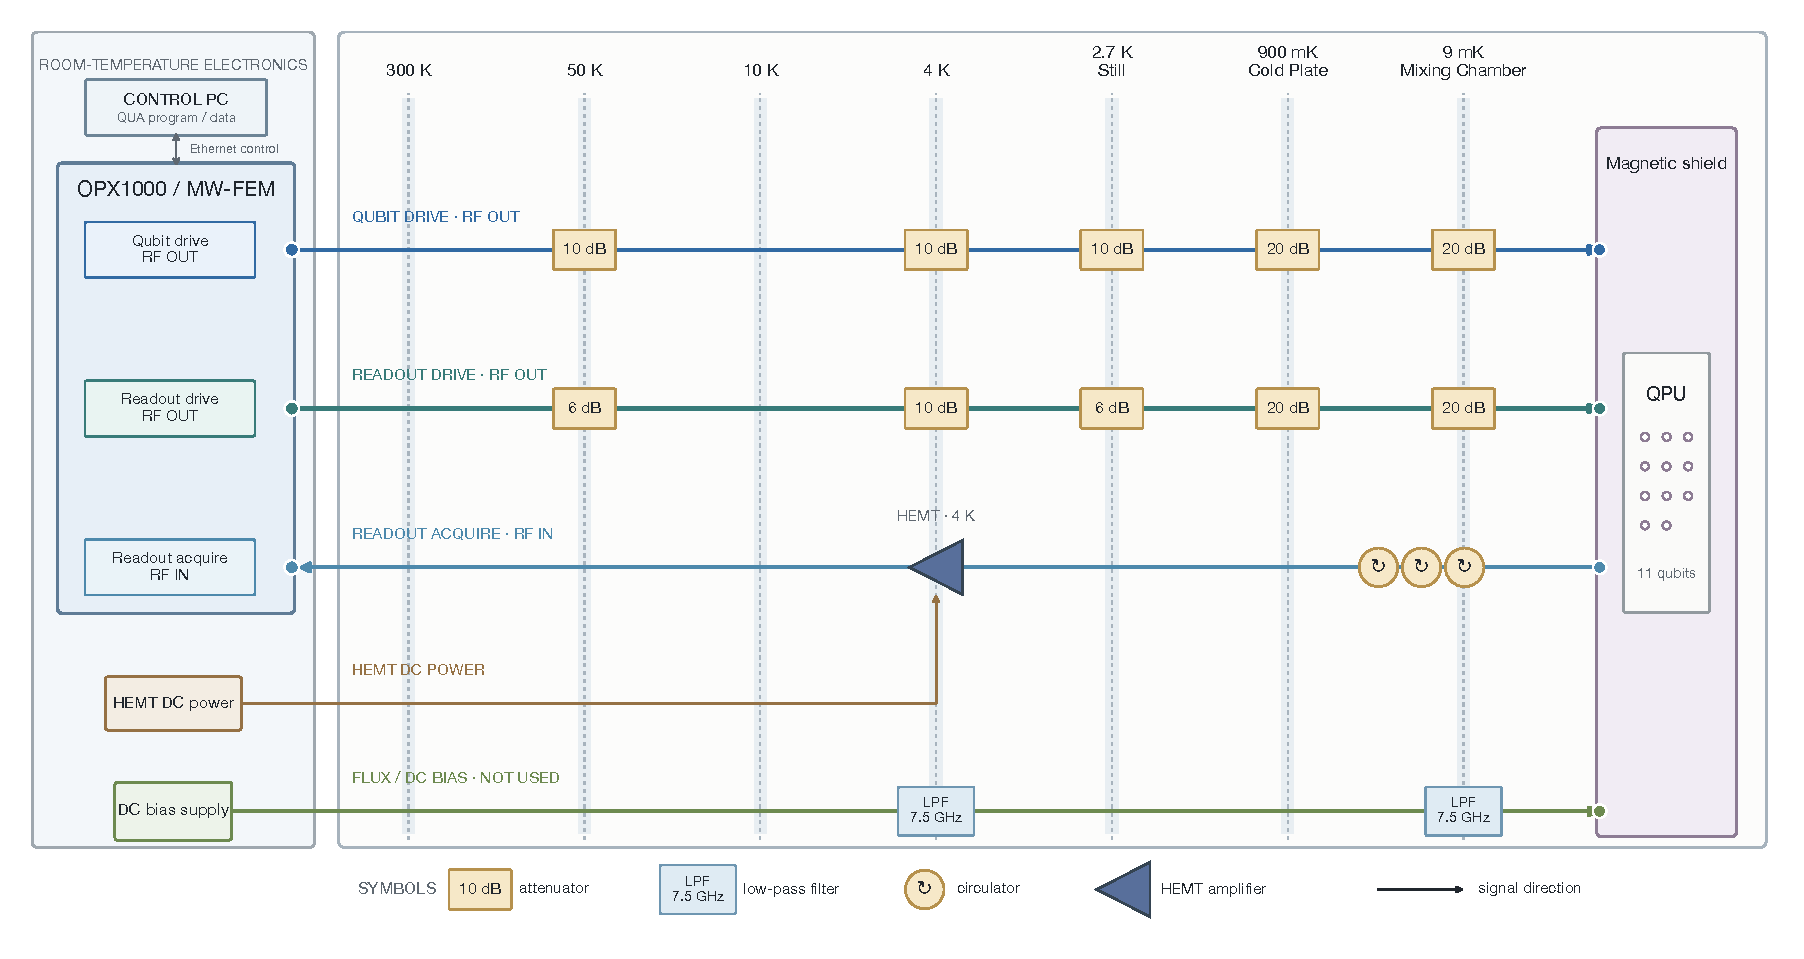
\includegraphics[width=0.98\linewidth]{figures/cryogenic_measurement_chain.pdf}
    \caption{Schematic of the experimental setup for qubit control and readout.
A control computer submits QUA programs and receives data over Ethernet.  The
OPX1000 MW-FEM directly generates the qubit-drive and resonator-readout RF
signals and acquires the returning readout signal.  Input lines are attenuated
across the 300 K, 50 K, 10 K, 4 K, still, cold-plate, and mixing-chamber stages.
The low-pass-filtered DC-bias line is shown for completeness but was not used.
At the mixing chamber, the device is isolated by circulators; the returning
readout signal is amplified by a 4 K HEMT before entering the MW-FEM for digital
downconversion and demodulation.}
    \label{fig:diagram}
\end{figure}

\subsection{Qubit coherence characterization}
\label{subsec:q1-coherence-characterization}

The energy-relaxation and Ramsey-dephasing times of the qubit used for the
spectroscopy measurements were characterized independently.  Figure~\ref{fig:q1-t1-t2}
shows representative measurements for qubit q1.  Fitting the excited-state
population to an exponential decay with a constant offset gives
$T_1=\MeasuredTOne~\mu\mathrm{s}$.  Fitting the positive-detuning Ramsey trace
to an exponentially damped sinusoid gives
$T_2^*=\MeasuredTTwoStar~\mu\mathrm{s}$.  The quoted uncertainties are
one-standard-deviation estimates obtained from the fit covariance matrices.
No associated Hahn-echo trace is available, so no measured Hahn-echo $T_2$ is
reported.  When one transverse time is required, we conservatively use
$T_{2,\mathrm{eff}}=T_2^*=\EffectiveTTwo~\mu\mathrm{s}$.  With the measured
$T_1$, this gives $T_\phi=\EffectiveTPhi~\mu\mathrm{s}$ through
$T_{2,\mathrm{eff}}^{-1}=(2T_1)^{-1}+T_\phi^{-1}$; this is not Hahn-echo
evidence.

\clearpage
\begin{figure}[t]
    \centering
    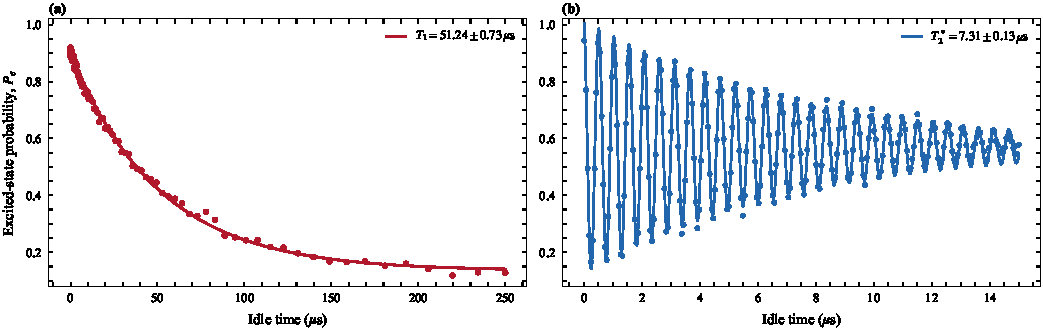
\includegraphics[width=\linewidth]{../figures/paper/05_q1_t1_t2.pdf}
    \caption{Independent coherence characterization of qubit q1.
    (a) Energy relaxation following state preparation, together with an
    exponential fit. (b) Ramsey fringes acquired with a positive
    $2~\mathrm{MHz}$ programmed detuning, together with an exponentially damped
    sinusoidal fit.}
    \label{fig:q1-t1-t2}
\end{figure}

\FloatBarrier

\section{Bloch-Equation Coherence Limit}
\label{sec:t2-limit}

For comparison with the shaped-pulse protocol, we first summarize the
steady-state response of a continuously driven two-level system.  We define
$w\equiv\rho_{00}-\rho_{11}$, with $\lvert0\rangle$ the ground state and
$\lvert1\rangle$ the excited state.  Hence $P_e=\rho_{11}=(1-w)/2$; no Pauli
matrix sign convention is left implicit.  Solving the optical Bloch equations for a drive
with angular Rabi frequency $\Omega_0$, angular detuning $\Delta$, relaxation
time $T_1$, and transverse coherence time $T_2$ gives~\cite{PhysRev.70.460}
\begin{equation}
    w_{\mathrm{ss}}(\Delta)
    =
    \frac{1+\Delta^2T_2^2}
    {1+\Delta^2T_2^2+\Omega_0^2T_1T_2},
    \qquad
    P_{e,\mathrm{ss}}(\Delta)
    =\frac{1}{2}
    \frac{s}{1+s+\Delta^2T_2^2},
    \quad s\equiv\Omega_0^2T_1T_2.
    \label{eq:bloch-steady-state}
\end{equation}
This expression assumes a pulse long enough to approach steady state.  It is a
reference result for conventional saturation spectroscopy, rather than a
closed-form description of the finite echo pulse.

At resonance, $P_{e,\mathrm{ss}}(0)=s/[2(1+s)]$, which approaches the
saturated value $1/2$ only for $s\gg1$.  The positive half-maximum detuning is
the angular-frequency HWHM
\begin{equation}
    \Delta_{\mathrm{HWHM}}
    =\frac{1}{T_2}\sqrt{1+s}.
    \label{eq:bloch-hwhm}
\end{equation}
The angular-frequency FWHM is therefore
\begin{equation}
    \Gamma_\omega
    \equiv 2\Delta_{\mathrm{HWHM}}
    =
    \frac{2}{T_2}
    \sqrt{1+s}.
    \label{eq:bloch-fwhm}
\end{equation}
The corresponding cyclic-frequency FWHM plotted in the Letter is
\begin{equation}
    \Gamma_f\equiv\frac{\Gamma_\omega}{2\pi}
    =\frac{1}{\pi T_2}\sqrt{1+s}.
    \label{eq:bloch-fwhm-hz}
\end{equation}
Thus $\Delta_{\mathrm{HWHM}}$, $\Gamma_\omega$, and $\Gamma_f$ are distinct
quantities and are not denoted by a common symbol.

In the weak-drive limit $s\ll1$,
\begin{equation}
    \Gamma_{\omega,T_2}=\frac{2}{T_2},
    \qquad
    \Gamma_{f,T_2}=\frac{1}{\pi T_2},
    \label{eq:t2-limited-angular-linewidth}
\end{equation}
which are the same coherence-limited FWHM expressed in angular frequency and
hertz, respectively.  In the strong-drive limit $s\gg1$,
\begin{equation}
    \Gamma_\omega
    \longrightarrow
    2\Omega_0\sqrt{\frac{T_1}{T_2}},
    \qquad
    \Gamma_f
    \longrightarrow
    2f_R\sqrt{\frac{T_1}{T_2}},
    \label{eq:power-broadened-linewidth}
\end{equation}
where $f_R=\Omega_0/(2\pi)$.  These limits are governed by $s$, not by
comparing $\Omega_0$ with an ambiguously defined linewidth.

\section{Pulse Truncation and Endpoint Amplitude}
\label{sec:pulse-cutoff}

The ideal Lorentzian tail has infinite support, whereas the implemented pulse
starts and ends at finite amplitude $\Omega_c=c\Omega_0$.  Abruptly switching
this residual drive produces an endpoint transient.  A useful estimate of the
associated population contribution is~\cite{mihov_defying_2024}
\begin{equation}
    P_c(\Delta)
    \simeq
    \frac{\Omega_c^2}{\Omega_c^2+\Delta^2}
    \left[1-P_0(\Delta)\right],
    \qquad \Omega_c=c\Omega_0,
    \label{eq:cutoff-artifact}
\end{equation}
where $P_0$ denotes the response that would be obtained without the endpoint
jump.  The artifact becomes important when $\Omega_c$ is comparable to the
linewidth scale of interest.  Thus the cutoff cannot be assessed from $c$
alone: it must be considered together with the peak drive and the desired
resolution.

The Bloch-equation reference gives the dimensionless endpoint saturation
parameter
\begin{equation}
    s_c=\Omega_c^2T_1T_2.
    \label{eq:cutoff-saturation}
\end{equation}
Keeping the endpoint contribution in the weak-saturation regime requires
\begin{equation}
    s_c\ll1
    \quad\Longleftrightarrow\quad
    \Omega_c\ll\frac{1}{\sqrt{T_1T_2}}
    \quad\Longleftrightarrow\quad
    c\ll\frac{1}{\Omega_0\sqrt{T_1T_2}}.
    \label{eq:cutoff-inequality}
\end{equation}
The inequality therefore bounds the endpoint amplitude from above.  It is a
perturbative design criterion, not a claim that the cutoff artifact has the
steady-state Lorentzian lineshape.

We therefore measured the cutoff dependence over two complementary q1
echo--root--Lorentzian scans.  The broad survey spans $c=0.002$--$0.99$
with 25 peak-amplitude settings, while the focused sweep resolves
$c=0.01$--$0.10$ with 200 peak-amplitude settings.  Both use a
$20~\mu\mathrm{s}$ pulse and the same measured transverse-coherence
reference, $T_2=6.856~\mu\mathrm{s}$.
Fig.~\ref{fig:echo-lorentzian-cutoff-sweep}
reports the dimensionless reciprocal-linewidth metric
\begin{equation}
    \mathcal{R}
    = \frac{\Gamma_{f,T_2}}{\Gamma_f}
    = \frac{1/(\pi T_2)}{\Gamma_f},
    \label{eq:cutoff-resolution-metric}
\end{equation}
where every linewidth is a cyclic-frequency FWHM in hertz.  Thus
$\mathcal{R}=1$ is the $T_2$-limited linewidth and
$\mathcal{R}<1$ denotes a broader feature.  We also show the
signal-weighted metric $|A_{\mathrm{fit}}|\mathcal{R}$, which suppresses
narrow fits with negligible contrast.  These are linewidth-based scores, not
direct estimates of frequency-estimation uncertainty.

The maps retain only resolved and bounded probability features: the fitted
contrast is between 0.05 and 1, $R^2\geq0.60$, the fitted center lies inside
the measured frequency interval, and the FWHM lies between two frequency bins
and half the sweep span.  Gray cells denote measurements for which the fit did
not pass this common screen.  The denser focused sweep provides substantially
more accepted fits than the coarse survey and resolves the loss of reciprocal
linewidth performance as the cutoff increases across the $0.01$--$0.10$
interval.

\begin{figure}[t]
    \centering
    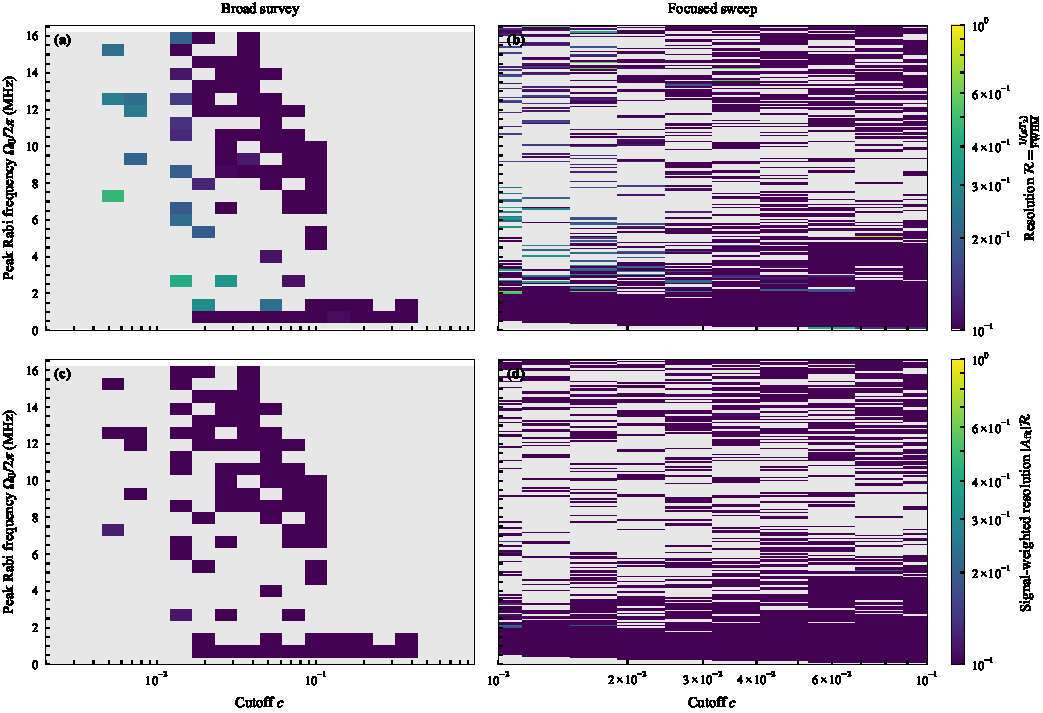
\includegraphics[width=\linewidth]{../figures/paper/08_echo_lorentzian_cutoff_sweep.pdf}
    \caption{Experimental cutoff sweep for q1 echo--root--Lorentzian
    spectroscopy.  The left column is the broad survey
    ($c=0.002$--$0.99$, 25 amplitudes, 60 repetitions per point); the right
    column is the denser focused sweep ($c=0.01$--$0.10$, 200 amplitudes,
    100 repetitions per point).
    (a,b) Reciprocal-linewidth metric $\mathcal{R}$ and
    (c,d) signal-weighted metric $|A_{\mathrm{fit}}|\mathcal{R}$.
    Both color scales are logarithmic.  On the upper color scale,
    $\mathcal{R}=1$ is the $T_2$-limited linewidth and values below one
    correspond to FWHM broader than that limit.  Gray cells are rejected or
    unresolved fits under the common screen described in the text; no fitted
    surface or interpolation is shown.}
    \label{fig:echo-lorentzian-cutoff-sweep}
\end{figure}
\FloatBarrier

\subsection{Simulated cutoff--amplitude operating map}

The finite-duration pulse is specified by its duration, peak drive amplitude,
and cutoff level.  To isolate the latter two parameters, we fix the pulse
duration at $50~\mu\mathrm{s}$ and simulate the root-Lorentzian and
echo-root-Lorentzian protocols over matched amplitude--cutoff grids.  For each
simulated spectrum, we extract the cyclic-frequency FWHM $\Gamma_f$ and the
contrast-weighted width
$\Gamma_f/(A_{\mathrm{peak}}\Gamma_{f,T_2})$.  This is a heuristic
resolution--signal metric; a direct Fisher-information or Cram\'er--Rao
analysis would additionally require a measurement-noise model and the full
frequency dependence of the response.

Fig.~\ref{fig:cutoff-parameter-map} shows that the root-Lorentzian pulse
contains extended narrow-linewidth regions, but its useful operating structure
is strongly oscillatory.  The echo protocol instead produces a broader,
contiguous region in which both the linewidth and the resolution--signal
trade-off remain favorable.  The logarithmic parameter axes should be kept in
mind when comparing the apparent area of these regions.

\begin{figure}[!ht]
    \centering
    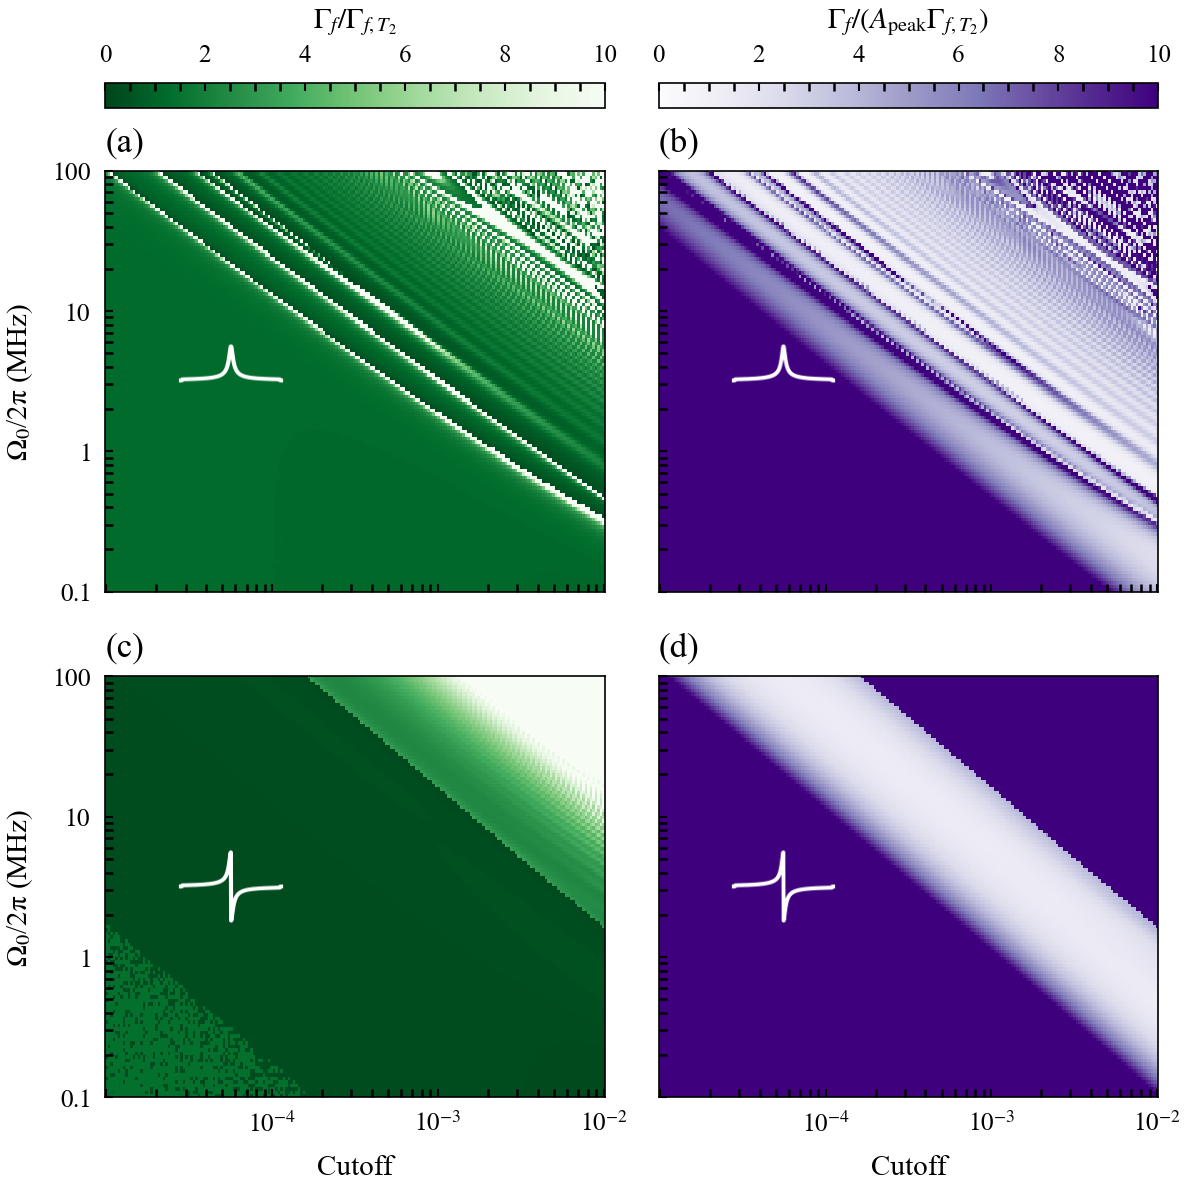
\includegraphics[width=0.72\textwidth]{../figures/paper/spectroscopy_fwhm_snr_vs_amplitude_vs_cutoff_2x2.png}
    \caption{Numerical cutoff--amplitude maps for root-Lorentzian $L^{(1/2)}$
    and echo-root-Lorentzian $L^{(1/2)}_{\mathrm{echo}}$ pulses of duration
    $50~\mu\mathrm{s}$.  (a,c) Normalized cyclic-frequency FWHM
    $\Gamma_f/\Gamma_{f,T_2}$ for the root and echo protocols, respectively;
    (b,d) corresponding contrast-weighted widths
    $\Gamma_f/(A_{\mathrm{peak}}\Gamma_{f,T_2})$.  The ordinary root-Lorentzian
    response is strongly oscillatory, whereas the echo variant retains a
    broader contiguous region with a favorable resolution--signal trade-off.}
    \label{fig:cutoff-parameter-map}
\end{figure}
\FloatBarrier

\section{Adiabatic Basis}
\label{sec:adiabatic-basis}


The matrix form of the Hamiltonian in the rotated frame takes the form:
\begin{equation}
    H(t) = \frac{1}{2}
    \begin{bmatrix}
            -\Delta & \Omega(t) \\ \Omega(t)  & \Delta
    \end{bmatrix}
\label{eq:rotated-hamiltonian-matrix}
.\end{equation}

The Rabi frequency $\Omega(t)$ quantifies the field-induced coupling between the two states. The instantaneous eigenstates of \( H(t) \), commonly referred to as the adiabatic states, are:
\begin{align}
| w_- (t) \rangle &= \cos \vartheta(t) |0\rangle - \sin \vartheta(t) |1\rangle, \\
| w_+ (t) \rangle &= \sin \vartheta(t) |0\rangle + \cos \vartheta(t) |1\rangle
\label{eq:rotating_basis}
,\end{align}
where the mixing angle is given by  $\vartheta(t) = \frac{1}{2}\arctan\frac{\Omega(t)}{\Delta}$. The corresponding eigenvalues, representing the adiabatic energy levels, are:
\begin{equation}
\varepsilon_{\pm}(t) = \frac{\hbar}{2} \left( \Delta \pm \sqrt{\Omega^2(t) + \Delta^2} \right)
,\end{equation}
yielding an energy gap of $\varepsilon(t) =\varepsilon_+(t) - \varepsilon_-(t) = \hbar \sqrt{\Omega^2(t) + \Delta^2}$.

Using the eigenvectors from Eq. (\ref{eq:rotating_basis}) we define the adiabatic transformation matrix $R$. Applying this transformation to the Hamiltonian in Eq. (\ref{eq:rotated-hamiltonian-matrix}) gives the  Hamiltonian in the adiabatic basis $H^{a} = R^{\dagger} H R - i R^{\dagger} \dot{R}$, which can be explicitly written as:



\begin{equation}
    H^a(t) = \frac{1}{2}
    \begin{bmatrix}
            -\varepsilon(t)/2 & -i\dot{\vartheta}(t) \\ \dot{\vartheta}(t)  & \varepsilon(t)/2
    \end{bmatrix}
    .
\end{equation}
Adiabatic evolution requires that the rate of change of the mixing angle \( \vartheta(t) \) is much smaller than the energy splitting $\varepsilon(t)$, leading to the adiabatic condition \cite{boradjiev_power_2013}:
\begin{equation}
| 2\dot{\vartheta}| \ll \varepsilon(t),
\label{eq:adiabatic-condition}
\end{equation}
where the non-adiabatic coupling term is given explicitly by $| \dot{\vartheta}| = \frac{\Delta\dot{\Omega}(t)}{2[\Delta+\Omega(t)]}$. 



\begin{figure}
    \centering
    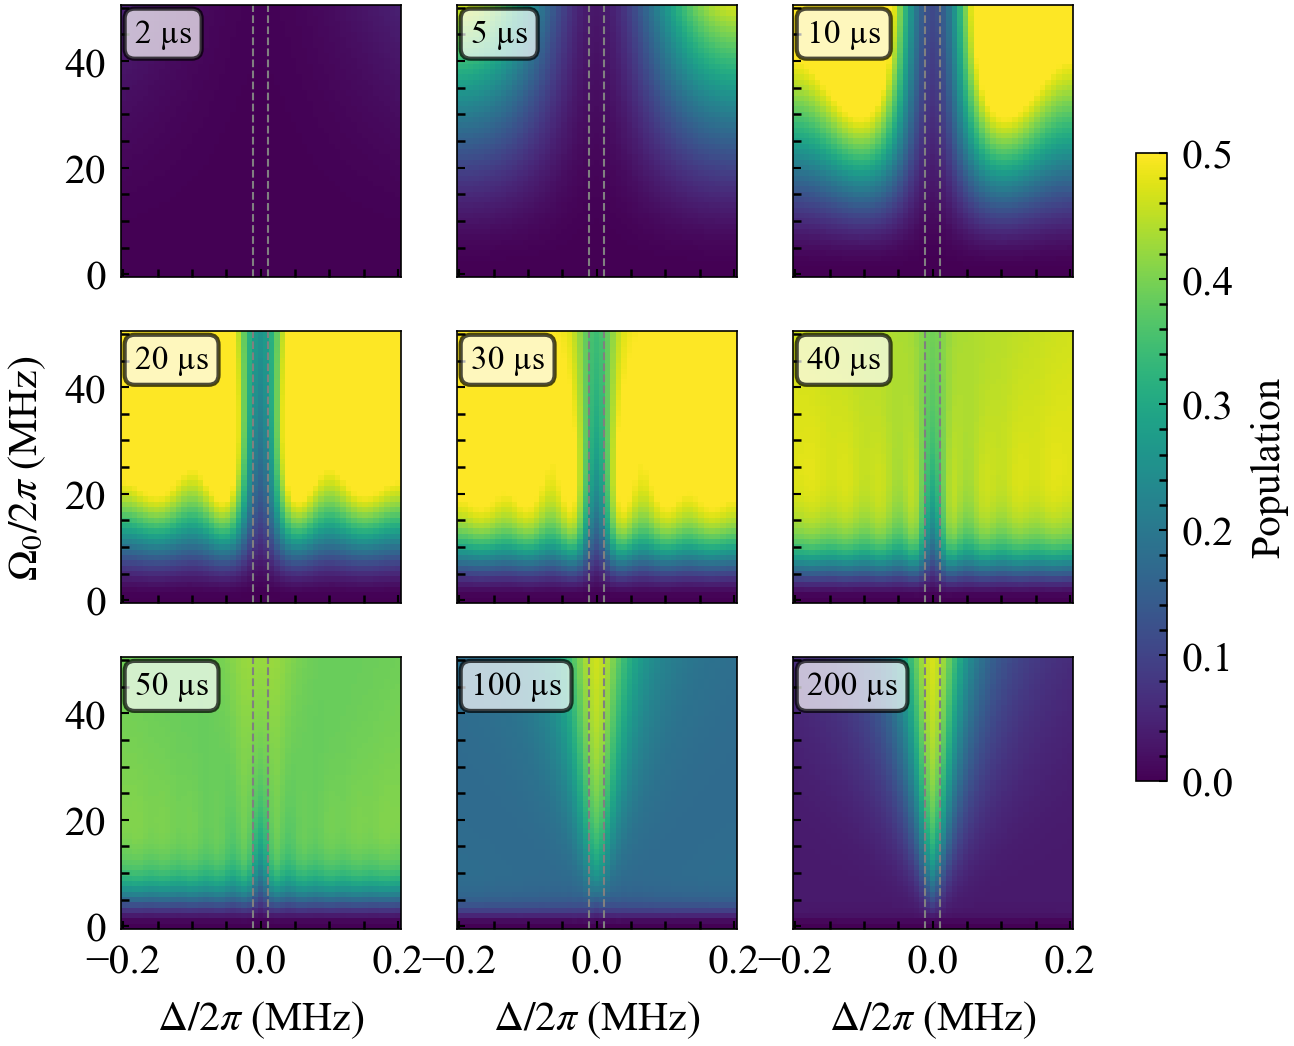
\includegraphics[width=1\linewidth]{figures/spectroscopy_length_comparison.png}
    \caption{Numerical spectroscopic response obtained using echo–root–Lorentzian pulses for different pulse durations (indicated in each panel). As the pulse length increases, the spectral linewidth progressively narrows, approaching the decoherence-limited resolution set by the coherence time $T_2$. For pulse durations comparable to or exceeding the relaxation time $T_1$, population decay during the interrogation leads to an elevated off-resonant background, reducing spectral contrast despite the continued narrowing of the resonance feature.}
    \label{fig:fig8}
\end{figure}




Replacing the inequality in Eq.  (\ref{eq:adiabatic-condition}) with an equality provides a approximate boundary condition between adiabatic  and non-adiabatic regions
\begin{equation}
   \sqrt{\Omega^2(t_0) + \Delta_b^2}= \frac{\Delta_b\dot{\Omega}(t_0)}{2[\Delta^2+\Omega^2(t_0)]}
,\end{equation}
where $t_0$ denotes the time at which the non-adiabatic coupling $| \dot{\vartheta}|$, is maximal, and  $\Delta_b$  marks the boundary between the adiabatic and non-adiabatic regimes. This condition allows us to extract a threshold value for the detuning range $\Delta<\Delta_b$ which marks the range of detunings where post-pulse excitation remains significant. The excitational linewidth scales proportionally to the threshold detuning  $\text{FWHM}\propto\Delta_b$. Consequently, we are particularly interested in the functional dependence of $\Delta_b$ on the peak Rabi frequency $\Omega_0$. 





\section{Pulse Length}
\label{sec:pulse-length}

The pulse duration imposes an additional constraint on spectroscopic resolution, as the spectral width of the drive in the frequency domain scales inversely with the pulse length. Figure 8 presents a numerical calculation of the extracted linewidth obtained using a square pulse, showing that for short pulse durations (  $\leq 20~\mu s$), the measured spectroscopic linewidth is dominantly limited by Fourier broadening rather than decoherence.

In contrast, for pulse durations exceeding approximately 20 $\mu s$, the echo-based pulse sequence approaches the decoherence-limited regime, yielding spectroscopy with an $\mathcal{O}(1)$ agreement with the $T_2$-limited linewidth.

For longer pulse durations, an additional effect emerges: the off-resonant background signal gradually decays while the resonance feature itself remains approximately constant. This results in the formation of a characteristic narrow peak nested within the broader echo-induced dip, reflecting the onset of adiabatic state evolution in the vicinity of the resonance.


\FloatBarrier
\section{Large-Drive Spectroscopy}
\label{sec:high-amplitude-regime}

\subsection{Broad and Narrow Frequency Scans}
\label{subsec:broad-and-narrow-scans}

High-resolution spectroscopy at large drive amplitudes is characterized on two
frequency scales.  A broad scan first locates the qubit transition and reveals
the surrounding baseline, nearby spectral features, and any strong-drive
distortions.  A narrow scan centered on the transition then samples the sharp
echo--root--Lorentzian depletion feature densely enough to determine its center
and linewidth.  Presenting the broad and narrow scans together distinguishes a
genuinely narrow resonance from a local feature embedded in a wider distorted
response and demonstrates that the high resolution persists within the full
spectral landscape.

\subsection{Extended-Amplitude Regime and Strong-Drive Distortions}
\label{subsec:extended-amplitude-regime}

At drive amplitudes above approximately $50~\mathrm{MHz}$, the Rabi frequency
is no longer small compared with the transmon anharmonicity and the measured
response begins to depart from an effective two-level description.  Possible
mechanisms include coupling
to higher transmon levels, drive-induced level shifts, leakage, and
multiphoton processes~\cite{PhysRevA.76.042319,motzoi_drag_2009,tuorila_stark_2010}.  The two-level calculation in
Sec.~\ref{sec:numerical-model} cannot distinguish among these mechanisms, so
the additional structure is reported here as a strong-drive distortion rather
than assigned to a specific transition.  Quantitative attribution would
require a converged multilevel model and an independent calibration of the
delivered drive amplitude.

\subsection{Cutoff Dependence from 50 to 80 MHz}
\label{subsec:high-amplitude-cutoff-comparison}

To separate large-drive behavior from changes in pulse duration or sampling,
we compare three q1 echo--root--Lorentzian scans acquired with the same
$10~\mu\mathrm{s}$ duration, detuning grid, amplitude grid, active-reset
protocol, and 40 repetitions per point.  Only the dimensionless cutoff-control
setting is changed, from $c=0.001$ to 0.005 and 0.010.  Using the same-day q1
$\pi$-pulse calibration retained with the data, the displayed portion of each
scan is selected from raw peak Rabi frequencies of $50.28$ to
$76.97~\mathrm{MHz}$.  The centers of the displayed block averages span
$50.67$ to $76.19~\mathrm{MHz}$.  This
restricted view exposes the high-amplitude response directly instead of
allowing the much larger low-amplitude region to dominate the color scale.
To reduce binomial sampling noise without imposing a fit or interpolated
surface, each displayed cell is a non-overlapping average of three adjacent
detuning points and three adjacent amplitude points.  Since every raw point
contains 40 repetitions, a displayed cell averages 360 binary outcomes.

Figure~\ref{fig:high-amplitude-cutoff-comparison} shows a pronounced
reorganization of the large-drive response with cutoff.  At $c=0.001$ the map
is dominated by a step-like change across zero detuning, whereas the
$c=0.005$ and 0.010 scans develop curved, amplitude-dependent fringes that
cross the central-frequency region.  Thus these measurements do not support
extrapolating the low-amplitude narrow-feature behavior unchanged into the
$50$--$80~\mathrm{MHz}$ regime.  Instead, they identify a cutoff-sensitive
strong-drive regime in which a single-linewidth description is insufficient.
Because all panels use one color scale, the differences are not artifacts of
independent normalization.

\begin{figure}[t]
    \centering
    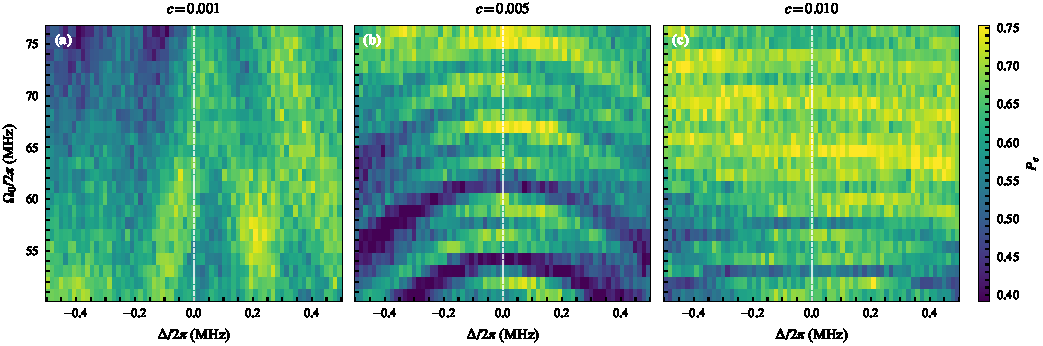
\includegraphics[width=1\linewidth]{../figures/paper/07_high_amplitude_cutoff_comparison.pdf}
    \caption{Measured high-amplitude echo--root--Lorentzian spectroscopy on
    q1 for dimensionless cutoff-control settings (a) $c=0.001$,
    (b) $c=0.005$, and (c) $c=0.010$.  Each panel shows the same
    $50.28$--$76.97~\mathrm{MHz}$ raw peak-Rabi-frequency interval from a
    $10~\mu\mathrm{s}$ scan with 40 repetitions per point.  The dashed line
    marks zero detuning, and all panels share the color scale.  Displayed cells
    are non-overlapping $3\times3$ block averages of the measured grid; no
    interpolation or fitted surface is shown.  The progression
    from a step-like response in (a) to curved interference fringes in (b) and
    (c) demonstrates that the large-drive structure is cutoff sensitive.}
    \label{fig:high-amplitude-cutoff-comparison}
\end{figure}
\FloatBarrier

\begin{figure}[t]
    \centering
    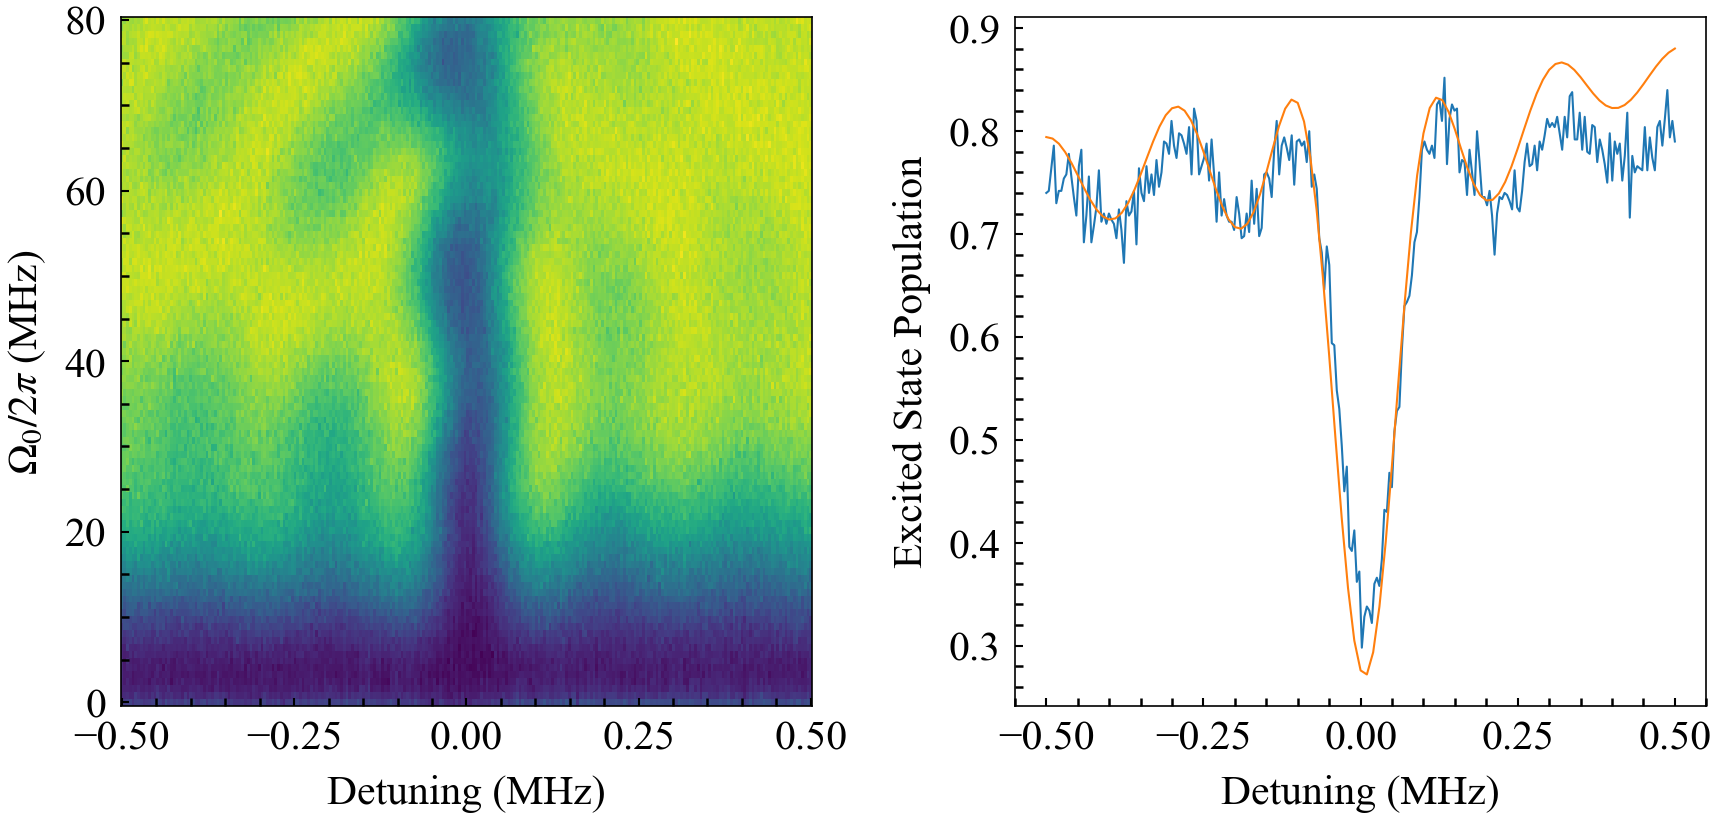
\includegraphics[width=1\linewidth]{figures/comparison.png}
    \caption{Two-dimensional spectroscopy map obtained with a
    $10~\mu\mathrm{s}$ echo--root--Lorentzian pulse at extended drive
    amplitudes (up to $80~\mathrm{MHz}$).  The left panel shows the full
    detuning--amplitude map, while the right panel presents a line cut at fixed
    drive strength (blue) together with a smooth fit (orange).  The observed
    distortions mark the breakdown of the ideal effective two-level response
    as the drive approaches the multilevel regime.}
    \label{fig:high-amplitude-comparison}
\end{figure}
\FloatBarrier

\section{Numerical Model}
\label{sec:numerical-model}

The simulations use an effective driven two-level system coupled to Markovian
relaxation and dephasing channels.  In the frame rotating at the drive
frequency, and within the rotating-wave approximation, the Hamiltonian is
implemented as
\begin{equation}
    \frac{H(t)}{\hbar}
    =
    \Delta a^\dagger a
    + \frac{\Omega_0}{2} f(t)
      \left(a+a^\dagger\right),
    \label{eq:numerical-hamiltonian}
\end{equation}
where $\Delta=\omega_q-\omega_d$ is the qubit--drive detuning, $\Omega_0$ is
the peak Rabi frequency, and $a=|0\rangle\langle1|$ is the lowering operator.
Up to an irrelevant identity term and the chosen sign convention for
$\Delta$, Eq.~\eqref{eq:numerical-hamiltonian} is equivalent to
$H/\hbar=(\Delta/2)\sigma_z+(\Omega_0 f/2)\sigma_x$.

For a root-Lorentzian pulse of total duration $L$, the dimensionless envelope
is
\begin{equation}
    f_{\mathrm{RL}}(t)
    =
    \left[1+\left(\frac{t}{\tau}\right)^2\right]^{-1/2},
    \qquad -\frac{L}{2}\le t\le\frac{L}{2},
\end{equation}
with $\tau$ chosen such that
$f_{\mathrm{RL}}(\pm L/2)=c$, where $c$ is the relative cutoff.  The echo
variant is obtained by changing the drive phase by $\pi$ at the pulse center,
\begin{equation}
    f_{\mathrm{ERL}}(t)
    = \operatorname{sgn}(-t) f_{\mathrm{RL}}(t).
    \label{eq:numerical-echo-envelope}
\end{equation}
The overall sign in Eq.~\eqref{eq:numerical-echo-envelope} is a phase
convention and does not affect the measured populations.

The density matrix evolves according to the Lindblad master equation
\begin{equation}
    \dot{\rho}
    =
    -\frac{i}{\hbar}[H(t),\rho]
    + \mathcal{D}\!\left[\sqrt{\frac{1}{T_1}}\,a\right]\rho
    + \mathcal{D}\!\left[\sqrt{\frac{2}{T_\phi}}\,
      a^\dagger a\right]\rho,
    \label{eq:numerical-master-equation}
\end{equation}
where
$\mathcal{D}[C]\rho=C\rho C^\dagger-\frac{1}{2}
\{C^\dagger C,\rho\}$ and
\begin{equation}
    \frac{1}{T_2}=\frac{1}{2T_1}+\frac{1}{T_\phi}.
\end{equation}
Each calculation starts in $|0\rangle$, integrates
Eq.~\eqref{eq:numerical-master-equation} over the complete pulse, and records
the final Bloch-vector components.  Spectroscopy maps are generated by
repeating this evolution over the experimental detuning and drive-amplitude
grids, using the pulse duration, cutoff, $T_1$, and $T_2$ associated with the
corresponding data set.

The numerical Hilbert space is restricted to two levels.  Consequently, this
model captures coherent drive dynamics, relaxation, and pure dephasing, but it
does not describe leakage, AC-Stark shifts produced by higher transmon levels,
or multiphoton transitions.  Comparisons in the extended-amplitude regime are
therefore interpreted as tests of where the effective two-level description
breaks down rather than as a simulation of those multilevel effects.

\section{Root-Lorentzian Versus Echo-Root-Lorentzian Pulses}
\label{sec:lorentzian-echo-comparison}

The two protocols are compared over the principal experimental control
parameters: pulse duration, relative cutoff, and peak drive amplitude.  For
each parameter set, we examine the final spectroscopic response, extracted
linewidth, signal contrast, and linewidth-to-signal ratio.  Pulse-length
sweeps distinguish the Fourier-limited and decoherence-limited regimes, while
cutoff sweeps quantify broadening introduced by truncating the formally
infinite Lorentzian tail.  Drive-amplitude sweeps then test whether the narrow
feature remains stable as the Rabi frequency is increased.  These comparisons
show where the phase inversion of the echo-root-Lorentzian pulse suppresses
coherent oscillations and produces a broader, more uniform operating region
than the corresponding root-Lorentzian pulse.

\section{Comparison Between Simulation and Experiment}
\label{sec:simulation-experiment-comparison}

Simulation and experiment are compared using the same final-state
spectroscopic observable and the same linewidth-extraction procedure.  The
comparison tests the resonance center, linewidth, and contrast across drive
amplitude, with the measured $T_1$ and $T_2$ supplied to the numerical model.
Agreement within the two-level operating range supports the proposed
echo-cancellation mechanism.  Systematic deviations at the largest amplitudes
identify the onset of physics omitted from the effective model, including
higher-level coupling and strong-drive calibration effects.


\bibliography{references}

\end{document}
